\subsection*{Functions Acting on Sets}
In our study of functions, we have focused on how a function ``maps'' individual elements of its domain to the codomain.  We also studied the preimage of an individual element in its codomain.  For example, if 
$f\x \mathbb{R} \to \mathbb{R}$ is defined by $f ( x ) = x^2$, for each 
$x \in \mathbb{R}$, then
\begin{itemize}
\item $f ( 2 ) = 4$.  We say that $f$ maps 2 to 4 or that 4 is the image of 2 under the function $f$.

\item Since $f ( x ) = 4$ implies that $x = 2$ or $x = -2$, we say that the preimages of 4 are 2 and $-2$ or that the set of preimages of 4 is $\left\{ -2, 2 \right\}$.
\end{itemize}

For a function $f\x S \to T$, the next step is to consider subsets of $S$ or $T$ and what corresponds to them in the other set.  We did this in the \typel activities.  We will give some definitions and then revisit the examples in the \typel activities in light of these definitions.  We will first consider the situation where $A$ is a subset of $S$ and consider the set of outputs whose inputs are from $A$.  This will be a subset of $T$.

\begin{defbox}{imageofA}{Let $f\x S \to T$\!.  If $A \subseteq S$, then the \textbf{image of 
$\boldsymbol{A}$ under $\boldsymbol{f}$}
\index{image!of a set}%
 is the set $f ( A )$, 
\label{sym:fofA} where
\[
f ( A ) = \left\{f ( x ) \mid x \in A \right\}\!.
\]
If there is no confusion as to which function is being used, we call $f ( A )$ 
\textbf{the image of $\boldsymbol{A}$}.}
\end{defbox}

We now consider the situation in which $C$ is a subset of $T$ and consider the subset of $A$ consisting of all elements of $T$ whose outputs are in $C$.

\begin{defbox}{inverseimage}{Let $f\x S \to T$.  If $C \subseteq T$, then the \textbf{preimage of $\boldsymbol{C}$ under $\boldsymbol{f}$}
\index{preimage!of a set}%
 is the set $f^{-1} ( C )$, 
\label{sym:preimage} where
\[
f^{-1} ( C ) = \left\{x \in S \mid f ( x ) \in C \right\}.
\]
If there is no confusion as to which function is being used, we call $f^{-1} ( C )$ \textbf{the preimage of $\boldsymbol{C}$}.  The preimage of the set $C$ under $f$ is also called the \textbf{inverse image of $\boldsymbol{C}$ under $\boldsymbol{f}$}\!.}
\index{inverse image of a set}%
\end{defbox}

\noindent
Notice that the set $f^{-1} ( C )$ is defined whether or not  $f^{-1}$ is a function.

\begin{prog}[\textbf{\typeu Activity~\ref*{PA:functionsandsets} Revisited}] \label{prog:functionsandsets} 
\hfill \\
Let $S = \left\{ a, b, c, d \right\}$ and $T = \left\{ s, t, u \right\}$.  Define $f\x S \to T$ by
\begin{align*}
f(a) &= s &  f(b) &= t &  f(c) &= t &  f(d) &= s.  \\
\end{align*}
\noindent
Let \quad $A = \left\{ a, c \right\}, \quad B = \left\{ a, d \right\},  \quad C = \left\{ s, t \right\},  
\quad \text{and} \quad D = \left\{ s, u \right\}$.

\noindent
Use your work in \typeu Activity~\ref*{PA:functionsandsets} to determine each of the following sets:

\begin{multicols}{4}
\begin{enumerate}
\item $f ( A )$
\item $f ( B )$
\item $f^{-1} ( C )$
\item $f^{-1} ( D )$
\end{enumerate}
\end{multicols}
\end{prog}
\hbreak

\begin{example}[\textbf{Images and Preimages of Sets}]\label{exam:imageandinverse} \hfill \\
Let $f\x  \mathbb{R} \to \mathbb{R}$ be defined by $f( x ) = x^2$, for each 
$x \in \mathbb{R}$.  The following results are based on the examples in 
\typeu Activity~\ref*{PA:functionsandsets} and \typeu Activity~\ref*{PA:functionsandint}.

\begin{itemize}
\item Let $A = \left\{ 1, 2, 3, -1 \right\}$.  Then
$f ( A ) = \left\{ 1, 4, 9 \right\}$.

\item Let $B = \left\{ 1, 9, 15, -1 \right\}$.  Then 
$f^{-1} ( B ) = \left\{ -\sqrt{15}, -3, -1, 1, 3, \sqrt{15} \right\}$.
\end{itemize}
%The graphs in Figure~\ref{fig:examplein91} will be used for the following:
%\begin{figure}[h]
%\begin{center}
%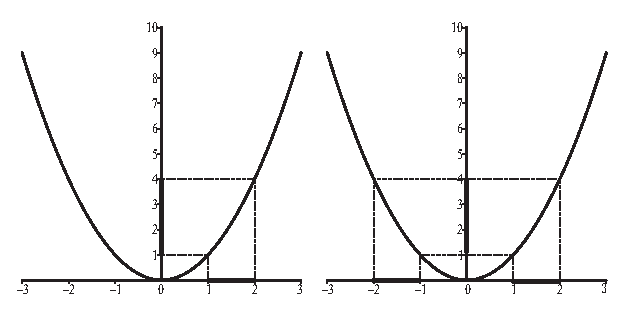
\includegraphics{figps-section9-1.eps} 
%\caption{Graphs for Example~\ref{exam:imageandinverse}} \label{fig:examplein91}
%\end{center}
%\end{figure}

%
\noindent
The graphs from \typeu Activity~\ref*{PA:functionsandint} illustrate the following results:
\begin{itemize}
\item If $T$ is the closed interval $\left[ 1, 2 \right]$, then the image of the set $T$ is
\[
\begin{aligned}
f ( T ) &= \left\{ f ( x ) \mid x \in \left[ 1, 2 \right] \right\} \\
                   &= \left[ 1, 4 \right]. \\
\end{aligned}
\]

\item If $C$ is the closed interval $\left[ 1, 4 \right]$, then the preimage of the set 
$C$ is
\[
\begin{aligned}
f^{-1} ( C ) &= \left\{ x \in \mathbb{R} \mid f ( x ) \in \left[ 1, 4 \right] \right\}
                        &= \left[ -2, -1 \right] \cup \left[ 1, 2 \right].
\end{aligned}
\]
\end{itemize}
\end{example}
\hbreak


\endinput
